В число стран-производителей, предоставляемых КиноПоиском, входит не только Россия, но и СССР, и Российская империя. Поэтому было решено рассмотреть фильмы, выпущенные не только в России, но и в предшествующих странах. У фильмов, выпущенных в период гражданской войны, указана страна «Россия», поэтому нельзя точно определить страну-производитель, используя только данные КиноПоиска. На графике на Рис.~\ref{fig:russia_rating} по оси абсцисс отложен год, а по оси ординат средний рейтинг по всем фильмам, выпущенным в этот год. Размер маркера прямопропорционален числу фильмов, выпущенных за конкретный год. Видно, например, что в СССР снимали меньше фильмов, но их рейтинг был лучше, чем у современных фильмов.

\begin{figure}[ht!]
	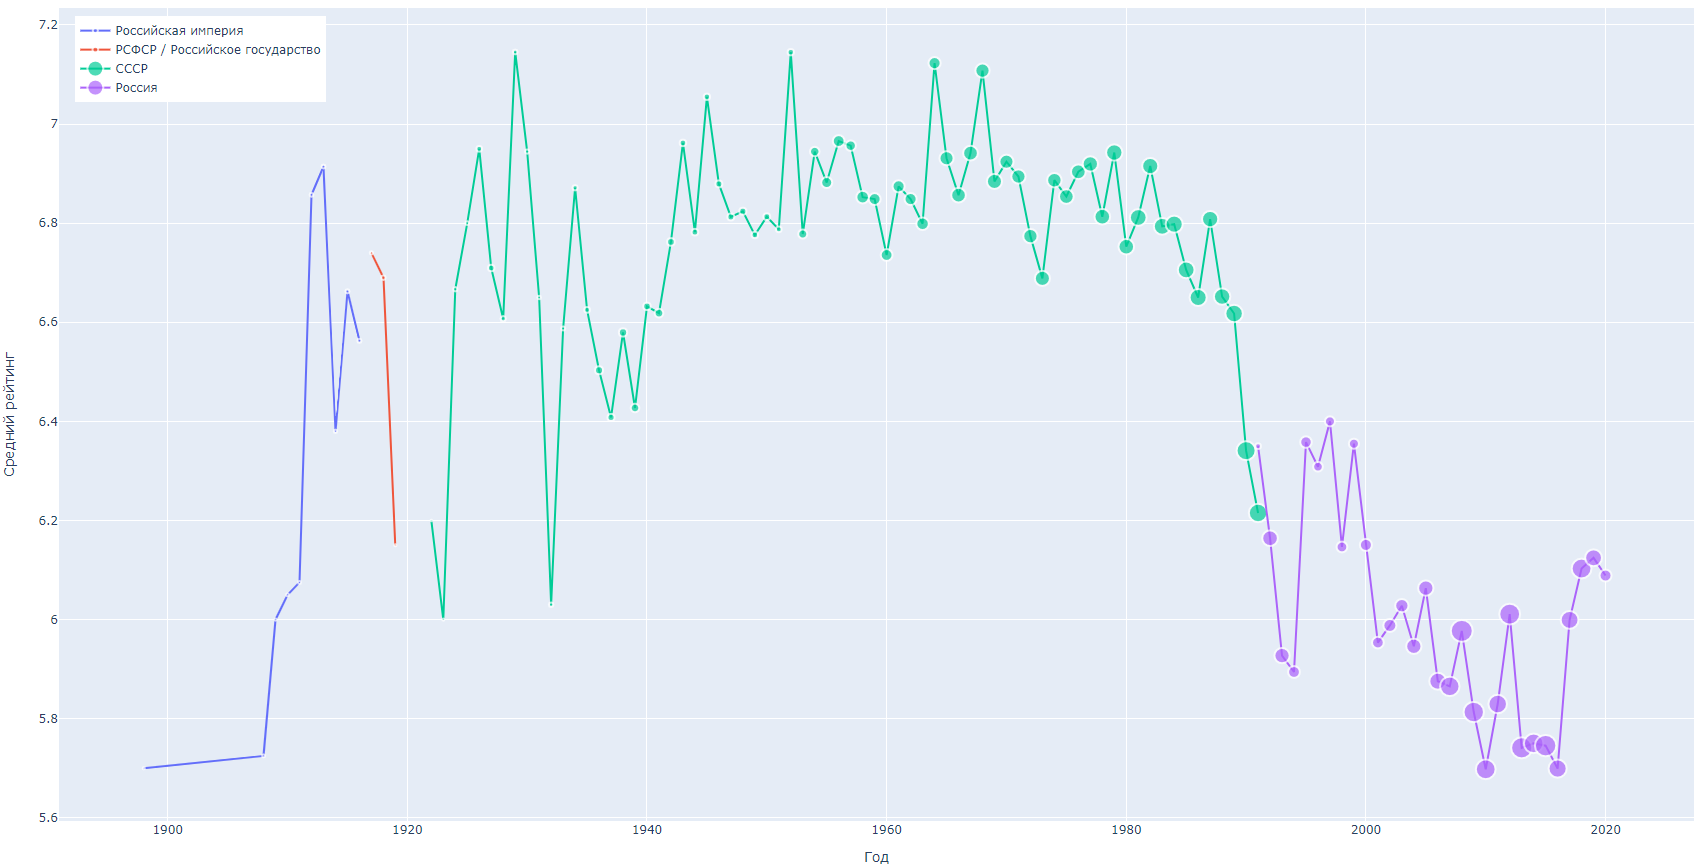
\includegraphics[width=\linewidth]{../report/images/russia_rating/1}
	\caption{Средний рейтинг российских фильмов по годам.}
	\label{fig:russia_rating}
\end{figure}


